%%
%% Class homework & solution template for latex
%% Alex Ihler
%%
\documentclass[twoside,11pt]{article}
\usepackage{amsmath,amsfonts,amssymb,amsthm}
\usepackage{graphicx,color}
\usepackage{verbatim,url}
\usepackage{listings}
\usepackage{upquote}
\usepackage[T1]{fontenc}
%\usepackage{lmodern}
\usepackage[scaled]{beramono}
%\usepackage{textcomp}

% Directories for other source files and images
\newcommand{\bibtexdir}{../bib}
\newcommand{\figdir}{fig}

\newcommand{\E}{\mathrm{E}}
\newcommand{\Var}{\mathrm{Var}}
\newcommand{\N}{\mathcal{N}}
\newcommand{\matlab}{{\sc Matlab}\ }

\setlength{\textheight}{9in} \setlength{\textwidth}{6.5in}
\setlength{\oddsidemargin}{-.25in}  % Centers text.
\setlength{\evensidemargin}{-.25in} %
\setlength{\topmargin}{0in} %
\setlength{\headheight}{0in} %
\setlength{\headsep}{0in} %

\renewcommand{\labelenumi}{(\alph{enumi})}
\renewcommand{\labelenumii}{(\arabic{enumii})}

\theoremstyle{definition}
\newtheorem{MatEx}{M{\scriptsize{ATLAB}} Usage Example}

\definecolor{comments}{rgb}{0,.5,0}
\definecolor{backgnd}{rgb}{.95,.95,.95}
\definecolor{string}{rgb}{.2,.2,.2}
\lstset{language=Matlab}
\lstset{basicstyle=\small\ttfamily,
        mathescape=true,
        emptylines=1, showlines=true,
        backgroundcolor=\color{backgnd},
        commentstyle=\color{comments}\ttfamily, %\rmfamily,
        stringstyle=\color{string}\ttfamily,
        keywordstyle=\ttfamily, %\normalfont,
        showstringspaces=false}
\newcommand{\matp}{\mathbf{\gg}}




\begin{document}

\centerline{\Large Homework 5}
\centerline{Zachary DeStefano, 15247592}
\centerline{CS 273A: Winter 2015}
\centerline{\bf Due: March 10, 2015}

\section*{Problem 1}

\subsection*{Part a}

The data does not look very clustered. Here is the plot of the raw data:

\begin{figure}[h]
\centering
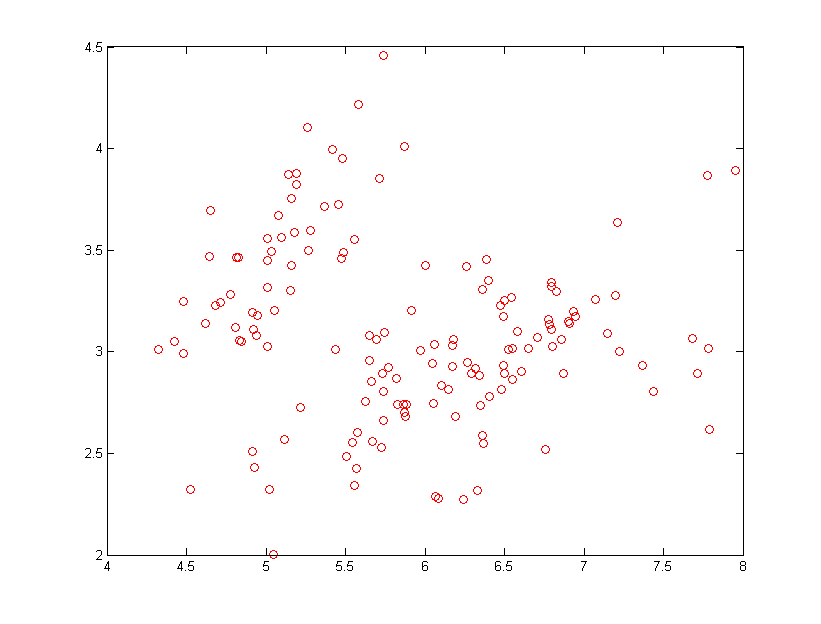
\includegraphics[width=6 in]{prob1PartA.png}
\caption{Raw Iris Data}
\end{figure}

\newpage

\subsection*{Part b}

Here are the clusters for $k=5$
\begin{figure}[h]
\centering
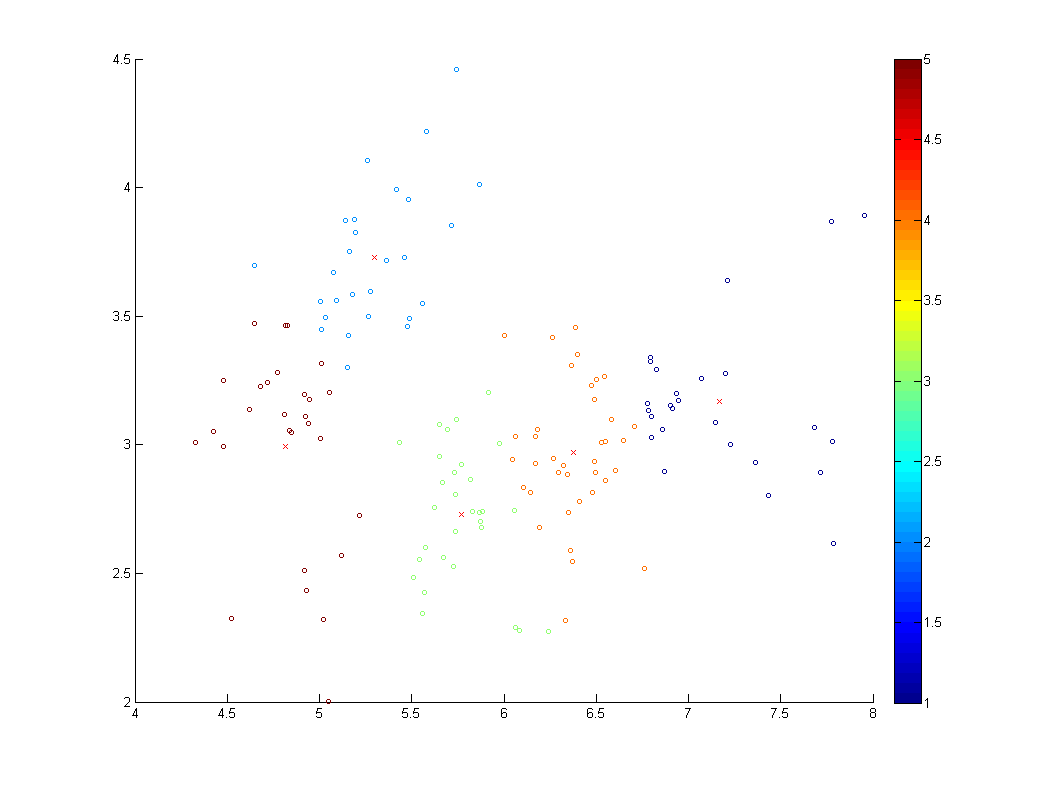
\includegraphics[width=6 in]{prob1PartB_1.png}
\caption{$k=5$ clustering with marked cluster centers}
\end{figure}

\newpage

Here are the clusters for $k=20$
\begin{figure}[h]
\centering
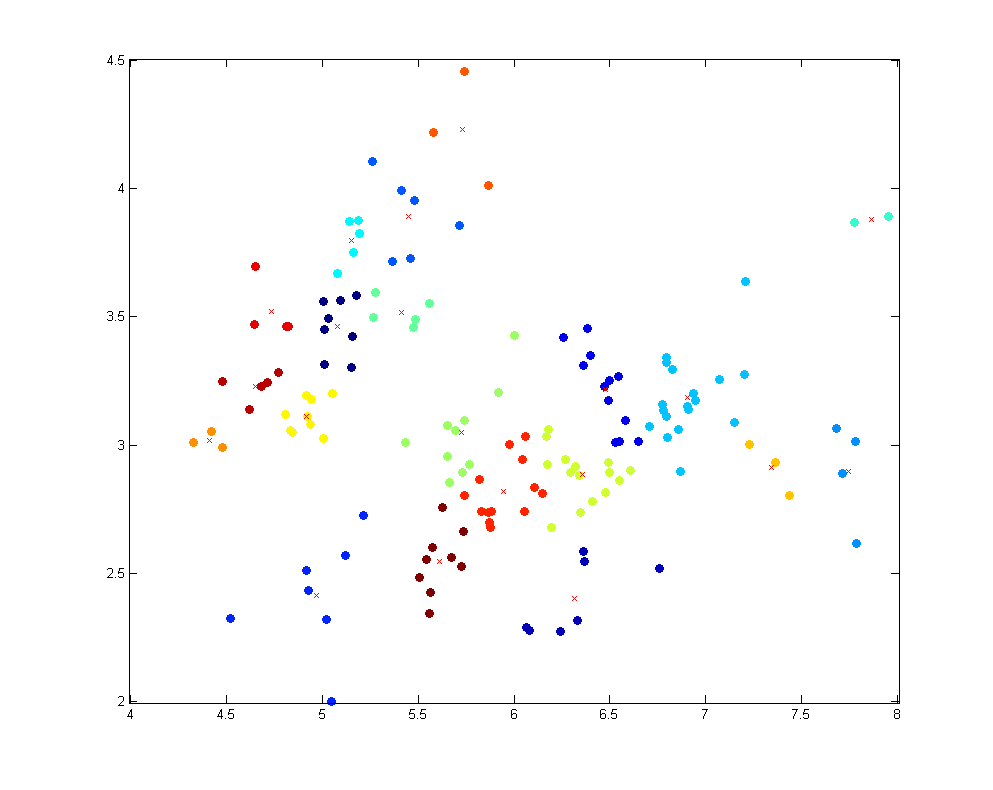
\includegraphics[width=6 in]{prob1PartB_2.png}
\caption{$k=5$ clustering with marked cluster centers}
\end{figure}

%\lstinputlisting[firstline=1, lastline=49]{prob1.m}



\end{document}
